%Dokumentinnstillinger:---------------------------------
%Ved å google flitting kan du finne ut hva de forskjellige tingene her betyr, og hvordan du kan gjøre eventuelle endringer.
\documentclass[a4paper,11pt,norsk]{article}
\usepackage[utf8]{inputenc}
\usepackage{a4wide}
\usepackage{lmodern}
\usepackage[T1]{fontenc}
\usepackage{babel}
\setlength{\parindent}{0pt} 
\setlength{\parskip}{2ex}
\usepackage{fixltx2e}
\usepackage{amsmath}
\usepackage[pdftex, pdfborderstyle={/S/U/W 0}]{hyperref}
\usepackage{graphicx}
\usepackage[font=small,labelfont=bf]{caption}
\usepackage{tabularx}
\usepackage{multirow}

\begin{document}

%Headingdel:---------------------------------------------
\begin{minipage}[c]{0.15\textwidth}

\includegraphics[width=2.0cm]{elsys_pos_staaende_ntnu}  
\end{minipage}
\begin{minipage}[c]{0.85\textwidth}

\renewcommand{\arraystretch}{1.7}
\large 
\begin{tabularx}{\textwidth}{|X|X|}
\hline
\multicolumn{2}{|l|}{} \\
\multicolumn{2}{|l|}{\huge \textbf{Designnotat}} \\
\multicolumn{2}{|l|}{}  \\
\hline
\multicolumn{2}{|l|}{Tittel: 
%Skriv inn tittel her:------------------------------------------
Hvordan lage en krets
} \\
\hline
\multicolumn{2}{|l|}{Forfattere: 
%Skriv inn forfattere her:--------------------------------------
Ola Normann og Kari Normann
} \\
\hline
%Skriv inn versjon og dato her her:-----------------------------
Versjon: 1.0 & Dato: 12.03.16
\\
\hline 
\end{tabularx}
\end{minipage}
\normalsize

%Automatisk generert innholdsfortegnelse:------------------

\setlength{\parskip}{0ex}
\renewcommand{\baselinestretch}{0.1}\normalsize
\tableofcontents
\renewcommand{\baselinestretch}{1.00}\normalsize
\setlength{\parskip}{2ex}
\rule{\textwidth}{1pt}

%Selve rapporten:------------------------------------------
\section{Problembeskrivelse}
\label{sec:innledning}

Se word-versjonen av designnotat-malen for beskrivelse av hva som skal være med i de forskjellige delene.

\section{Prinsipiell løsning}
\label{sec:prinsipielllosning}

Blablabla. Løsningen er basert på kretsen i~\cite[s. 1604]{bibelen}. Slik som dette refererer vi altså til bibliografien. Videre ser vi av formelen
\begin{equation}
  \label{eq:formel}
  x = \frac{-b \pm \sqrt{b^{2}-4ac}}{2a}
\end{equation}
at bla bla bla. Vi kan også referere til likning (\ref{eq:formel}) igjen.

\section{Realisering og test}
\label{sec:realisering}

Målinger av $c_0$, $v_1$ og $v_2$ er vist i figur~\ref{fig:resultat}.
\begin{figure}[htbp]
  \centering
  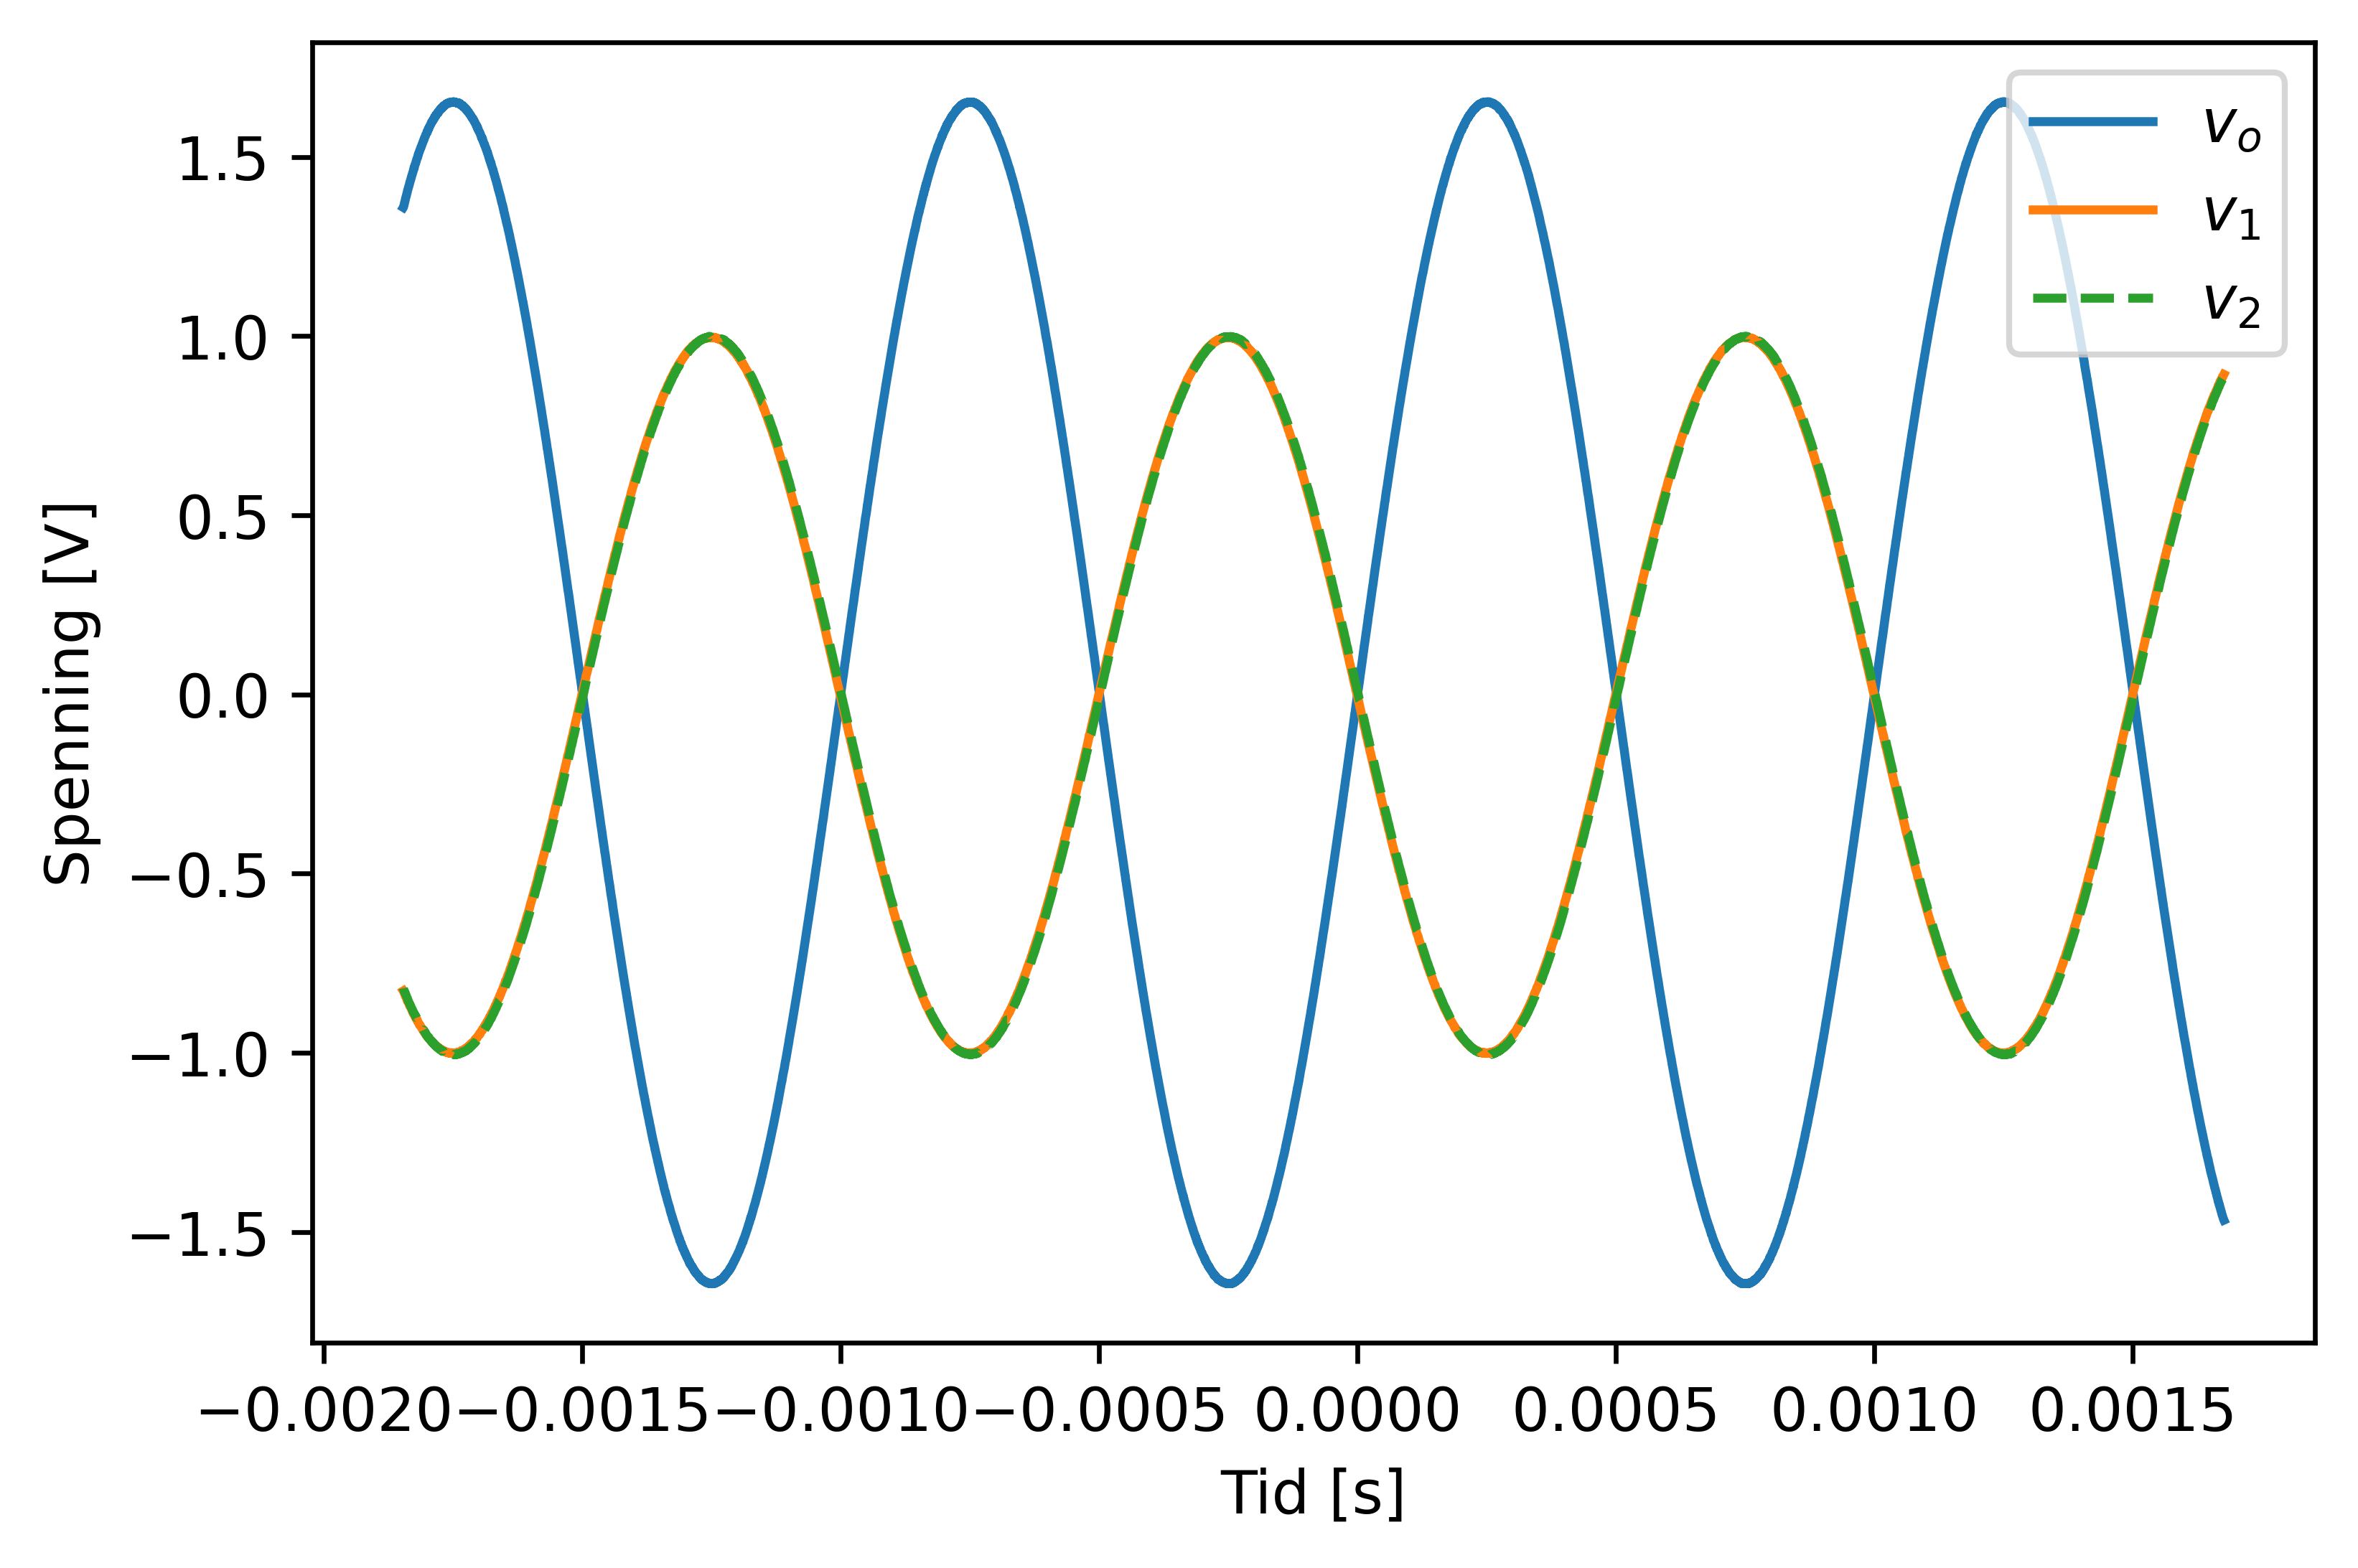
\includegraphics[width=0.6\textwidth]{skop} 
  \caption{Inngang $v_1$ (blå kurve) og utgang $v_2$ (grønn).}
  \label{fig:resultat}
\end{figure}

Slik setter vi altså inn en figur og refererer til den. 

Vi kan også kryssreferere til f.eks. seksjon~\ref{sec:prinsipielllosning} ved å bruke labels.



\section{Konklusjon}
\label{sec:konklusjon}

Blablabla. ... som er innenfor 10\% av kravet.

\section{Takk}
Blablabla.

%Bibliografi: Legg til flere elementer ved å legge til flere \bibitem:--------
\phantomsection
\addcontentsline{toc}{section}{Referanser}
\begin{thebibliography}{99}

\bibitem{bibelen}
  Albert Einstein,
  \emph{Elektronikkbibelen},
  O Store Forlag,
  1. utgave,
  1930.

\end{thebibliography}

\appendix
%Tillegg. Flere tillegg legges til ved å lage flere sections:-----------------
\section{Ekstra greier}
Mindre relevant blabla.


\end{document}